\documentclass[12pt]{article}
\usepackage{tikz}

\usepackage{graphicx, titling, amsmath, amsthm, amsfonts, amssymb, algorithm, algpseudocode}
\graphicspath{{./images/}}

\renewcommand\maketitlehooka{\null\mbox{}\vfill}
\renewcommand\maketitlehookd{\vfill\null}

\title{DS 221 - Assignment 3}
\author{Shankaradithyaa Venkateswaran\\ Sr no: 22190}
\date{\today}

\begin{document}
\begin{titlepage}
    \maketitle
\end{titlepage}

\section*{Note to Professor}
I am sorry for the late submission, actually while I went for the results verification I realized I had submitted the wrong report pdf. This is my actual report for the assignment, and I hope that it is considered for grading over my old one.

\section*{Question 1}
\subsection*{Methodology}
For the first question, we had to code an OpenMP program to calculate the prefix sum of a problem. Here I follow a simple parallel algorithm of the prefix sum problem. This is to take the input array and split it between n number of threads then run the standard prefix sum algorithm on each thread.
\begin{verbatim}
    Parallel for each thread from 0 to num_threads - 1:
        Get thread id (tid)
        Calculate start index (start) for this thread
        Calculate end index (end) for this thread

        If start index is within bounds:
            Set B[start] to A[start]
            For each index i from start + 1 to end - 1:
                Set B[i] to B[i - 1] + A[i]
\end{verbatim}
After calculating the prefix sum in each thread, I calculate the offset for each part of the array and then I add this offset to get the global prefix sum of the array.
\begin{verbatim}
    Initialize offsets array with size num_threads and all elements set to 0
    For each thread from 1 to num_threads - 1:
        Set offsets[thread] to offsets[thread - 1] + B[thread * chunk_size - 1]

    Parallel for each thread from 0 to num_threads - 1:
        Get thread id (tid)
        Calculate start index (start) for this thread
        Calculate end index (end) for this thread

        If thread id is greater than 0 and start index is within bounds:
            For each index i from start to end - 1:
                Set B[i] to B[i] + offsets[tid]
\end{verbatim}
To create the array, I use the following code:
\begin{verbatim}
    std::srand(std::time(0)); // Seed for random number generation
    std::vector<int> A(n);
    for (int i = 0; i < n; ++i) {
        A[i] = std::rand() % 10001; // Random integers between 0 and 10000
    }
\end{verbatim}

\subsection*{Results}
I was asked to run the program for n = 10000, 20000, and 30000 with 1, 2, 4, 8, 16, 32, and 64 threads. I use a shell script to run the code. For each combination, I run the program 5 times and average the reults to obtain the following:\\
\begin{table}[h!]
    \centering
    \begin{tabular}{|c|c|c|}
        \hline
        \textbf{Threads} & \textbf{Execution Time (seconds)} & \textbf{Speedup} \\
        \hline
        1 & 9.9988e-05 & 1.0 \\
        \hline
        2 & 0.000144407 & 0.6924041078341079 \\
        \hline
        4 & 0.00020233119999999997 & 0.49417983978743774 \\
        \hline
        8 & 0.000312018 & 0.3204558711356396 \\
        \hline
        16 & 0.0005224308 & 0.191389941021854 \\
        \hline
        32 & 0.03739564 & 0.0026737876394146484 \\
        \hline
        64 & 0.002319138 & 0.0431142950527308 \\
        \hline
    \end{tabular}
    \caption{Execution times and speedups for different thread counts with array size 10000}
    \label{table:results}
\end{table}\\
The graphs for the same are as follows:
\begin{center}
    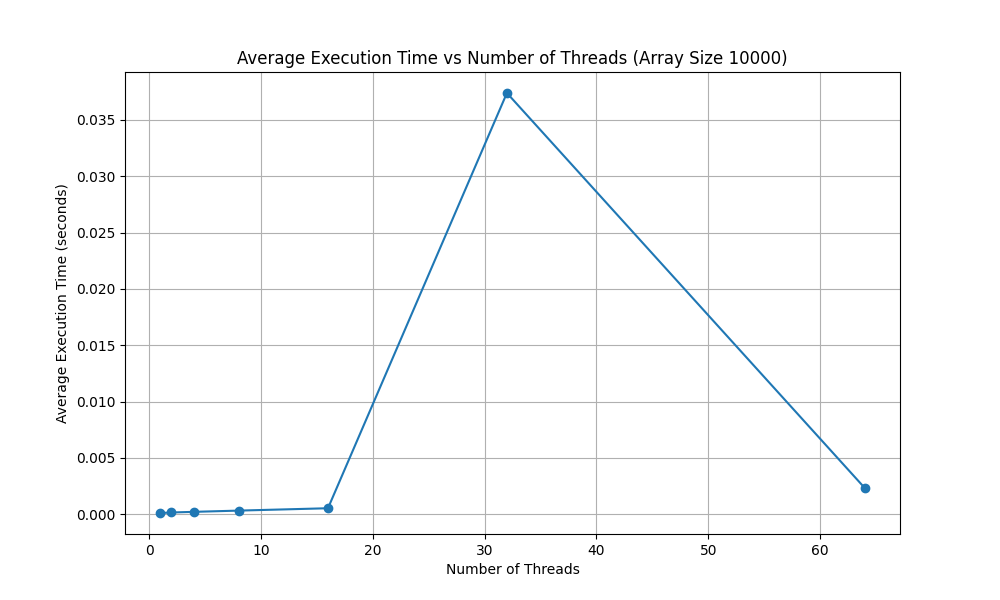
\includegraphics[width=0.8\textwidth]{execution_time_vs_threads_10000.png}
    \label{fig:10000}
\end{center}

\begin{center}
    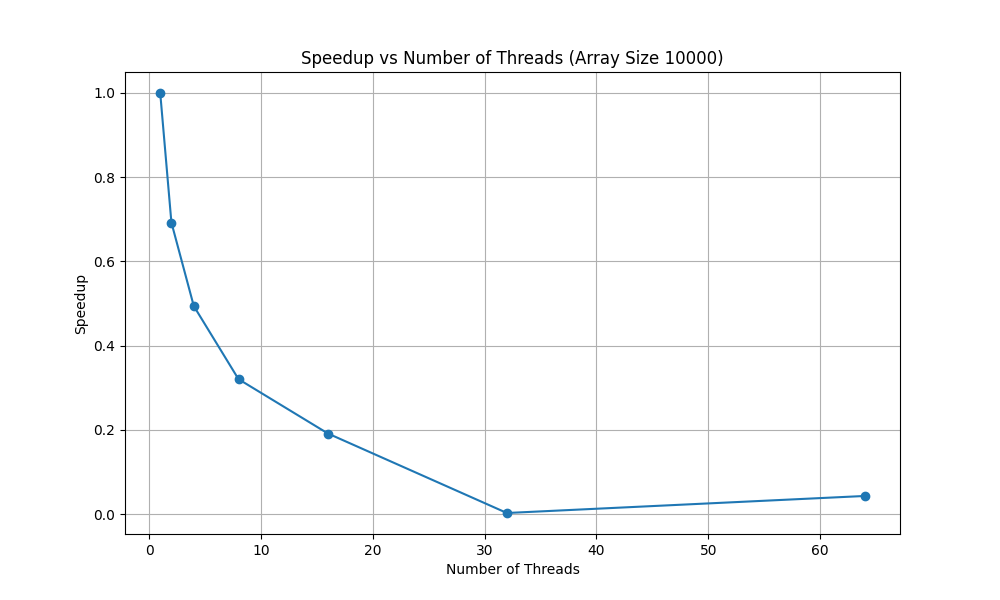
\includegraphics[width=0.8\textwidth]{speedup_vs_threads_10000.png}
    \label{fig:10000}
\end{center}

\begin{table}[h!]
    \centering
    \begin{tabular}{|c|c|c|}
    \hline
    \textbf{Threads} & \textbf{Execution Time (seconds)} & \textbf{Speedup} \\ \hline
    1  & 0.000192167  & 1.0 \\ \hline
    2  & 0.0002166514 & 0.8869871138612536 \\ \hline
    4  & 0.0002929936 & 0.6558743945260238 \\ \hline
    8  & 0.00034444   & 0.5579113924050633 \\ \hline
    16 & 0.0005522474 & 0.34797266587402675 \\ \hline
    32 & 0.03605448   & 0.005329906297358886 \\ \hline
    64 & 0.002256242  & 0.08517127152140595 \\ \hline
    \end{tabular}
    \caption{Execution Times and Speedups for Array Size 20000}
    \label{table:execution_times_speedups}
\end{table}
The graphs for the same are as follows:
\begin{center}
    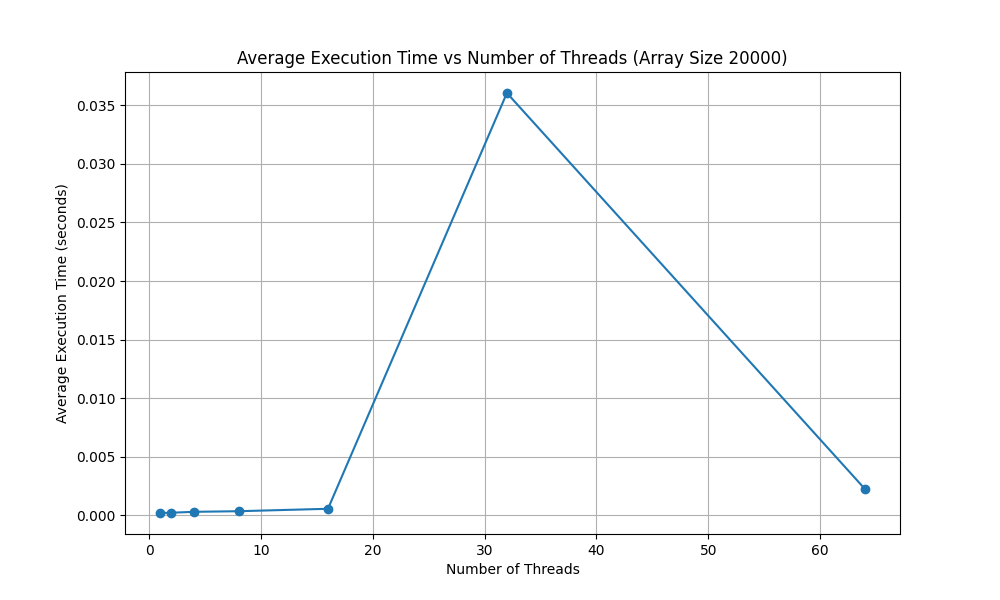
\includegraphics[width=0.8\textwidth]{execution_time_vs_threads_20000.png}
    \label{fig:20000}
\end{center}

\begin{center}
    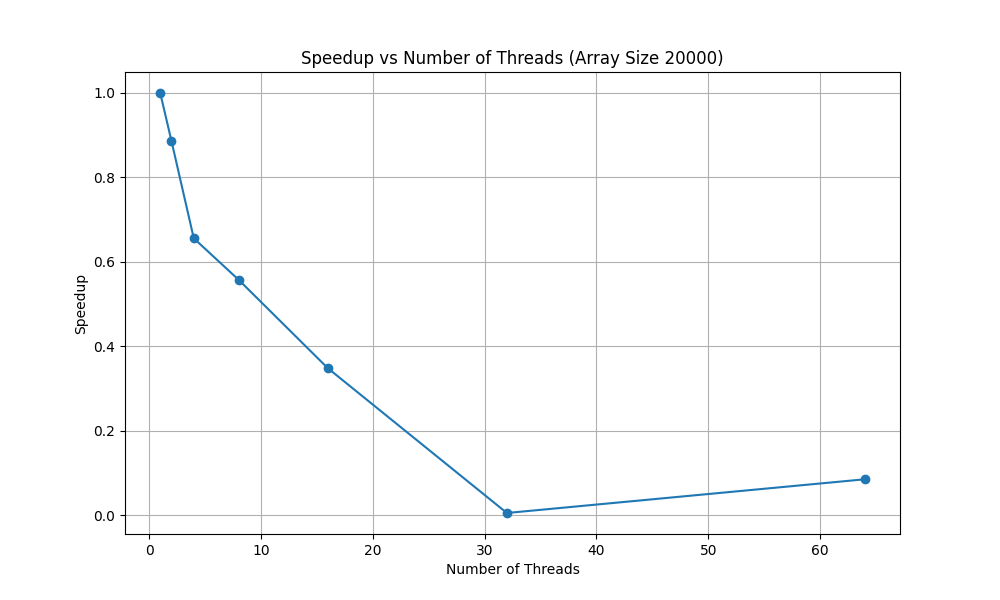
\includegraphics[width=0.8\textwidth]{speedup_vs_threads_20000.png}
    \label{fig:20000}
\end{center}

\begin{table}[h!]
    \centering
    \begin{tabular}{|c|c|c|}
    \hline
    \textbf{Threads} & \textbf{Execution Time (seconds)} & \textbf{Speedup} \\ \hline
    1  & 0.0002634672  & 1.0 \\ \hline
    2  & 0.0003021140  & 0.8720787517294797 \\ \hline
    4  & 0.0003121138  & 0.8441382598270246 \\ \hline
    8  & 0.0003700024  & 0.7120688946882507 \\ \hline
    16 & 0.0006018374  & 0.43777139805535525 \\ \hline
    32 & 0.0437044     & 0.006028390734113729 \\ \hline
    64 & 0.002524538   & 0.10436254078964154 \\ \hline
    \end{tabular}
    \caption{Execution Times and Speedups for Array Size 30000}
    \label{table:execution_times_speedups_30000}
\end{table}
The graphs for the same are as follows:
\begin{center}
    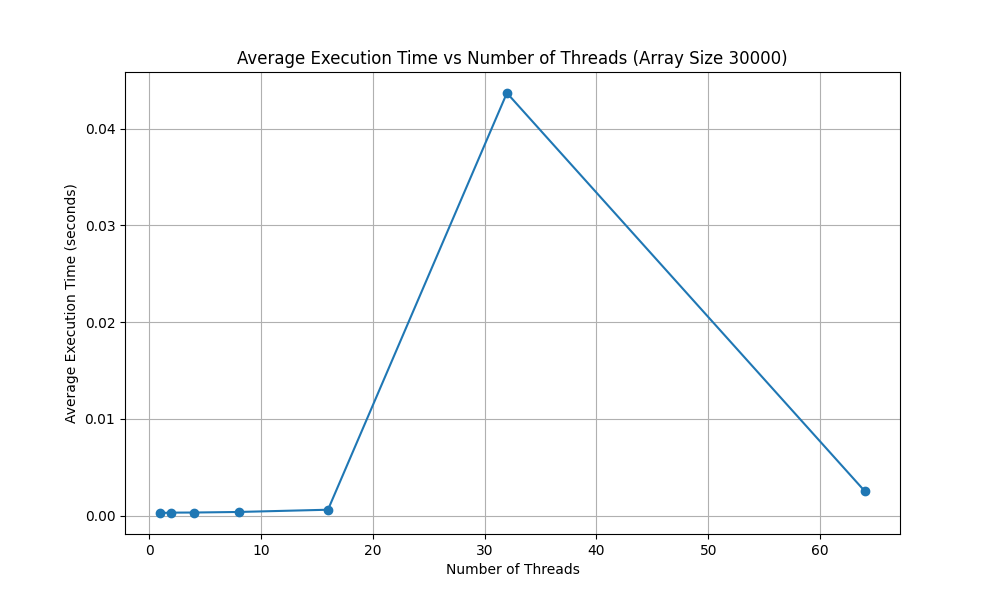
\includegraphics[width=0.8\textwidth]{execution_time_vs_threads_30000.png}
    \label{fig:30000}
\end{center}

\begin{center}
    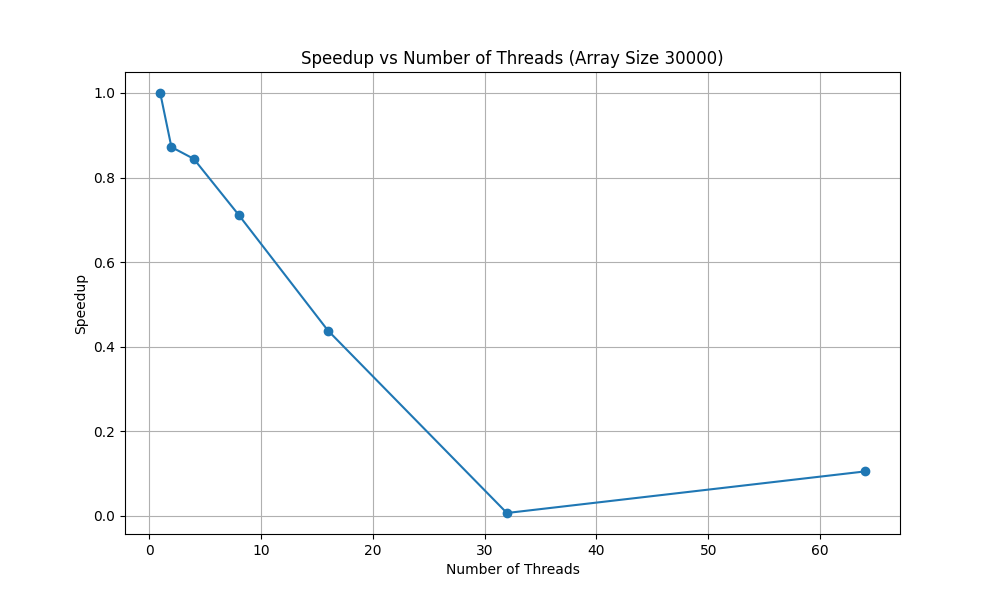
\includegraphics[width=0.8\textwidth]{speedup_vs_threads_30000.png}
    \label{fig:30000}
\end{center}

\subsection*{Analysis}
From the results, we can see that execution time is approximately the same as the threads start to increase, and at 32, it shoots up as the overhead of the parallelization is too much. But as we increase it a little more, we can see that at 64 threads it is much faster than 32 threads. We can see that the speedup is not linear as the number of threads increases. This is because of the overhead of creating threads and managing them. The speedup is maximum at 2 threads and then starts to decrease as the number of threads increases. This is because the overhead of creating threads is more than the speedup we get from parallelizing the code. But from the results we can see that the speedup for 64 threads is more than for 32, but it is still decreasing almost linearly. We can say this because parallelizing only for the order of 10,000s is not worth it as the overhead is too much. But we can say that for larger arrays, parallelizing the code is worth it as the speedup will be more than 1.

\section*{Question 2}
\subsection*{Methodology}
For the second question, we were tasked with writing an MPI code for finding an element in an array. Here I follow a simple algorithm to split up the 1000000 element array between the number of processes and then run a simple linear search to find the element in the array.
\begin{verbatim}
    Broadcast element_to_find to all processes

    Calculate chunk_size as (n + size - 1) / size
    Calculate start as rank * chunk_size
    Calculate end as (start + chunk_size < n) ? start + chunk_size : n
    
    Initialize found to 0
    Initialize local_index to -1
    
    // Each process searches in its subarray
    for i from start to end - 1 do
        if A[i] equals element_to_find then
            found = 1
            local_index = i
            break
        end if
    end for
\end{verbatim}
If a process has found the element, it sends a found message to all other processes. Now if the element is not in process 0, I call MPI REDUCE to get the global index of the element. After all this, process 0 prints the global index of the element.
\begin{verbatim}
    Share the found status among all processes
    global_found = MPI_Allreduce(found, MPI_LOR)
    
    If any process found the element, update the global index
    global_index = -1
    if global_found then
        global_index = MPI_Reduce(local_index, MPI_MAX, 0)
    
    Process 0 prints the result
    if rank == 0 then
        print "Element to find: " + element_to_find
        if global_index != -1 then
            print "Global index of element " 
            + element_to_find + " is: " 
            + global_index
        else
            print "Element " + element_to_find + " not found in the array."
\end{verbatim}
I use the following code to create the array, broadcast it to all processes, and generate a random element to find in the array.
\begin{verbatim}
    const int array_size = 1000000;
    int* A = (int*)malloc(array_size * sizeof(int));

    if (rank == 0) {
        // Seed the random number generator with a combination of current 
        time and rank
        srand(time(0) + rank + clock());
        // Generate random integers between 1 and 5000000
        for (int i = 0; i < array_size; ++i) {
            A[i] = rand() % 5000000 + 1;
        }
    }

    double start_time = MPI_Wtime(); // Start time

    // Broadcast the array from process 0 to all other processes
    MPI_Bcast(A, array_size, MPI_INT, 0, MPI_COMM_WORLD);

    int n = array_size;

    // Generate a random element to search for
    int element_to_find;
    if (rank == 0) {
        srand(time(0) + clock()); // Reseed the random number generator
        element_to_find = rand() % 5000000 + 1;
    }
\end{verbatim}

To run all this code, I use Slurm along with a shell script and use sbatch to run the code as a batch job. The node on the cluster can only support 32 processes, hence I need to ask for 2 nodes so that each process has a different core. I use the following parameters to run the code:
\begin{verbatim}
    #SBATCH --nodes=2
    #SBATCH --cpus-per-task=1
    #SBATCH --ntasks=64
    #SBATCH --time=10:00:00
\end{verbatim}

\subsection*{Results}
I was asked to run the code for an array size of 1000000 with elements varying from 1 to 5000000. This was to be run for 1, 2, 4, 8, 16, 32, and 64 processes, 20 times each, and it should be averaged out. The averaged results are as follows:
\begin{table}[h!]
    \centering
    \begin{tabular}{|c|c|c|}
    \hline
    \textbf{Processes} & \textbf{Speedup} & \textbf{Average Execution Time (seconds)} \\ \hline
    1  & 1.0                        & 0.16163975 \\ \hline
    2  & 2.7389882808263746         & 0.0590144 \\ \hline
    4  & 3.5939791195804793         & 0.04497515 \\ \hline
    8  & 13.660255137181657         & 0.011832850000000002 \\ \hline
    16 & 5.9754037303818555         & 0.027050849999999998 \\ \hline
    32 & 44.55401810940064          & 0.003627949999999999 \\ \hline
    64 & 87.88351230120972          & 0.0018392500000000002 \\ \hline
    \end{tabular}
    \caption{Speedups and Average Execution Times for Different Numbers of Processes}
    \label{table:speedups_execution_times}
\end{table}
The graphs for the same are as follows:
\begin{center}
    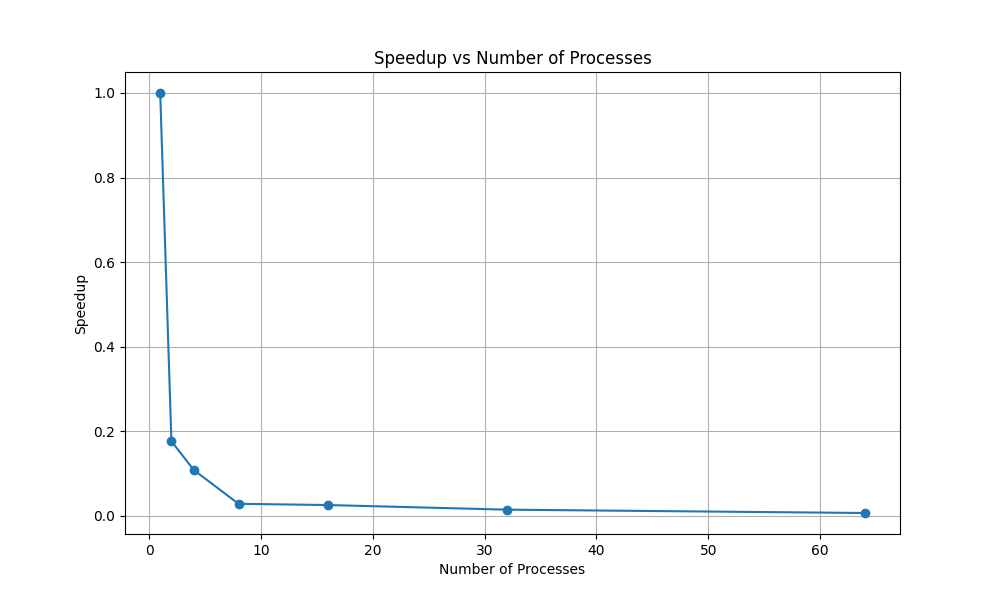
\includegraphics[width=0.8\textwidth]{speedup_vs_processes.png}
    \label{fig:speedup_processes}
\end{center}

\begin{center}
    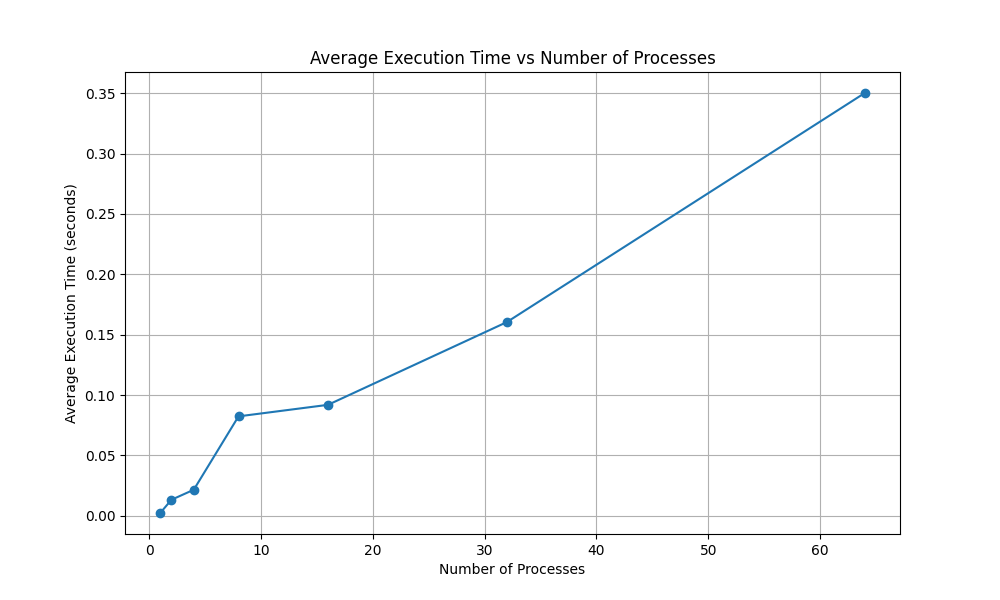
\includegraphics[width=0.8\textwidth]{avg_execution_time_vs_processes.png}
    \label{fig:execution_time_processes}
\end{center}

\subsection*{Analysis}
From the graph we can see that speedup is decreasing greatly as the number of processes increases. This is because of the overhead of creating processes, and passing the data to them is a lot more than the increase in execution time provided by the actual parallelism. As noted the execution time is increasing as the number of processes increase. I am measuring time taken including the broadcast times.
\end{document}